\chapter{Cronograma de execução do projeto}

O projeto para a construção do HGTD está dividido em diferentes frentes de trabalho, onde cada frente é responsável pelo desenvolvimento de um componente específico do sistema. O grupo HEPIC estará focado no desenvolvimento do sensor LGAD em conjunto com as colaborações ATLAS e RD50. 

%Atualmente a pesquisa com o LGAD está sendo desenvolvida por uma colaboração de 24 institutos de 12 países, ligados ao experimento ATLAS. Esses institutos, incluindo o Instituto de Física da Universidade de São Paulo, serão responsáveis por desenvolver a tecnologia necessária para a produção dos dispositivos que serão empregados na construção do HGTD.

Como mostra a Fig. \ref{cronograma}, em vermelho, o plano de execução para o desenvolvimento do LGAD tem a duração total de seis anos (2019 - 2025), onde estão inclusas as fases de desenvolvimento do sensor; início de 2019 até o início de 2022, e produção dos dispositivos; de 2022 até o início de 2025. 

Neste contexto, como dito anteriormente no texto desta proposta, o projeto terá duas frentes de trabalho paralelo, uma dedicada aos trabalhos de desenvolvimento para o ATLAS, e outra para o desenvolvimento de sensores semicondutores e suas diversas aplicações no Brasil. Como mostra a Fig. \ref{cronograma}, a barra azul mostra o período aproximado de execução deste projeto o qual terá duração de três anos com início em 2020 e término em 2023, podendo claramente ser estendido de acordo com os compromissos assumidos durante esse período e a disponibilidade de recursos.

%Como pode ser visto no gráfico \ref{cronograma}, a execução do projeto é dividida em três etapas onde inicialmente
O planejamento prevê o estabelecimento da infraestrutura para executar as medidas dos parâmetros do dispositivo. Essa fase, representada pela cor marrom, é comum para as duas etapas seguintes, e será trabalhada até a primeira metade de 2020 onde o comissionamento de diversos equipamentos será feito. Em seguida duas outras etapas serão executadas em paralelo, e são representadas pelas cores purpura e verde no gráfico. Em purpura está representada as atividades dedicadas ao desenvolvimento do LGAD para o experimento ATLAS, onde estão previstas as atividades de desenvolvimento e certificação dos sensores seguindo o planejamento traçado pelo ATLAS.

E em verde tem se listado os detalhes para a produção e utilização dos sensores empregando os arranjos experimentais que serão desenvolvidos no Brasil, beneficiando-se do conhecimento adquirido em colaboração com o ATLAS.

Por fim, os principais milestones do projeto são mostrados em sua linha do tempo. De acordo com este cronograma, é importante destacar que a produção dos primeiros protótipos do LGAD no Brasil é esperada para ser concluída no início de 2022, marcando a obtenção da tecnologia e das ferramentas necessárias para a produção deste sensor no Brasil. Em seguida, após uma fase de aperfeiçoamento do sensor e do sistema de aquisição de dados, o dispositivo estará completamente integrado em 2022, completando o ciclo de desenvolvimento das ferramentas necessárias para a construção de um sistema de detecção de raios-X de alta precisão para a medida de energia, posição e tempo, e também capaz de medir intervalos de tempo muito curtos da ordem de pico segundos.

\begin{figure}
    \centering
    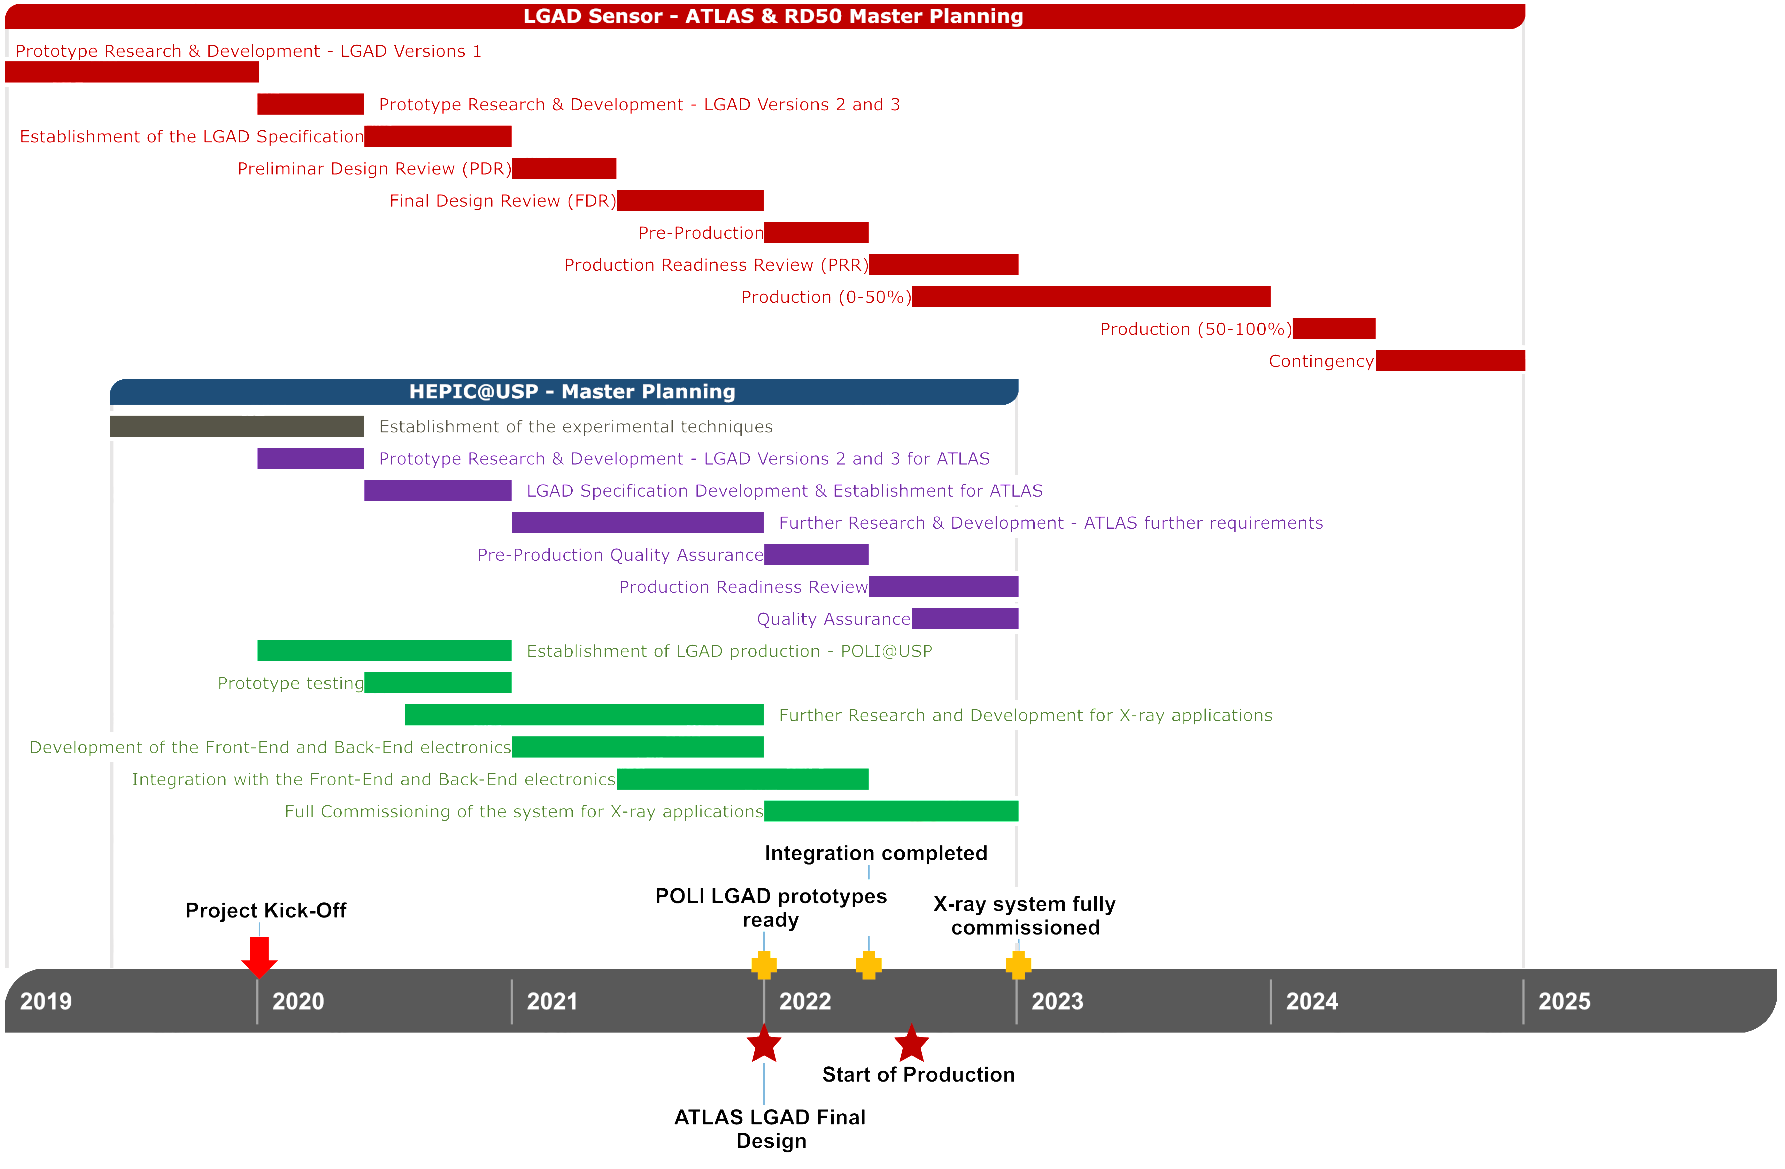
\includegraphics[width=18.0cm]{assets/cronograma.png}
    \caption{Gráfico mostrando o planejamento para o desenvolvimento do LGAD, incluindo as revisões do projeto (PDR, FDR, PRR), pré-produção e produção. Abaixo da barra azul temos o plano que será desenvolvido no HEPIC@USP visando o desenvolvimento do LGAD e suas aplicações. Os principais {\it milestones} do projeto são mostrados em sua linha do tempo.}
    \label{cronograma}
\end{figure}